\chapter{Clang Analysis}

\section{Introduction}

In this chapter it will be described the analysis process for all the tools used.\newline\newline
\textbf{Understand} is indeed the tools that gives the most accurate results in terms of checks, since it incorporates C/C++ MISRA standards, a beta version of the \textbf{CLang Static Analyzer}, which is a static analysis tool provided by the LLVM developers, and many other quality checks offered by SciTools itself.\newline
A simpler but also quite effective tool is \textbf{Cppcheck} which is designed to "provide unique code analysis to detect bugs and to focus on detecting undefined behaviour and dangerous coding constructs" \cite{bibitem2}. Also, as pointed by the developers, its main focus is to  "detect only real errors in the code (i.e. have very few false positives)". Cppcheck refers to the \textsl{Common Weakness Enumeration} standard for the analysis, a formal list of security issues published by the MITRE institute. It is also possible to check MISRA-C project compliance but it requires to buy the standard so this feature was not used. \newline
The last used tool is \textbf{flawfinder} which puts its focus more on security flaws rather than quality issues. This tool incorporates an option to run the analysis in order to detect possible false positives in an automated manner. This tools uses the CWE standard as Cppcheck does.\newline
Other tools such as \textbf{SonarQube} and \textbf{Cert C Rosechecker} were used but due to their characteristics they were unusable for our purpose.
\pagebreak

\section{Analysis Methodology}

The LLVM Clang compiler was analized with all the tools listed above.\newline
Since some issues arose while analyzing the whole project, as it was pointed in the previous section, a representative subset of it was chosen. In particular the folder \textbf{src/tool/libclang} was analyzed because it has been observed that the source files in this folder contained much of the compiler logic. This was the input folder for all the static analysis tools used.\newline\newline
After the output was produced, the second phase of the analysis can start. Since the output format of the various tool is hetherogenous, it was necessary to convert them in excel sheets in order to collect evidences about what files were the most vulnerable/contained more bugs.

\section{Understand}

Understand is a very powerful tool for static analysis that can be used to analyze software written in multiple languages suchs as Java, Ada, Cobol, Python, C/C++\dots
Among the tools used, it is the only one that comes with a nice and user-friendly user interface that allows users to navigate through the software files.

\subsection{Understand Project}

First of all, it must be created an \textsl{Understand Project}. In this first step you are asked to select the language of the software (C/C++ in our case study) and the directories to analyze.\newline\newline
\vspace{1cm}
\begin{minipage}{\linewidth}
	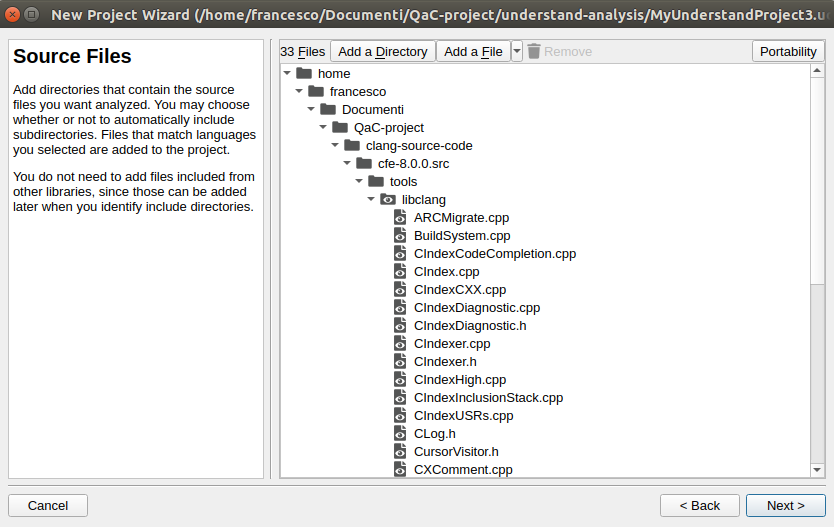
\includegraphics[width=\textwidth]{img/libclangDirectory.png}
	\captionof{figure}{The whole subdirectory tools/libclang is imported in the Understand project in order to run the analysis.}
\end{minipage}

When the files are loaded in the program, the analysis can be run simply by opening the \textsl{codecheck perspective} and selecting which standard should guide it.\newline\newline
\vspace{1cm}
\begin{minipage}{\linewidth}
	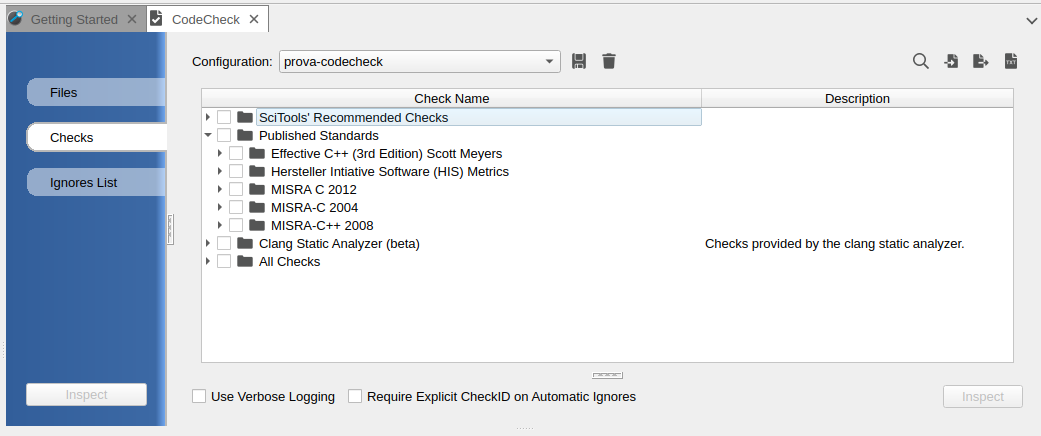
\includegraphics[width=\textwidth]{img/Codecheck.png}
	\captionof{figure}{The MISRA standard is incorporated in Understand, as well as the Clang Static Analyzer. Generic checks are also offered by the tool as \textsl{SciTools Recommended Checks} and \textsl{AllChecks}, some of which are redundant.}
\end{minipage}

\begin{itemize}
	\item \textsl{SciTools' Recommended Checks} - This is a small set (17 items) of generic good programming rules
	\item \textsl{Published Standards} - This section contains the published standards supported by Understand
		\begin{itemize}
			\item It was used the MISRA-C++ 2008 due to the nature of the source files (.cpp) and because one of the goals of this project was to check the Clang compiler compliance to MISRA rules.
		\end{itemize}
	\item \textsl{Clang Static Analyzer} - Is an implementation of the tool incorporated in Understand.
	\item \textsl{All Checks} - This is a collection of checks which consists of generic good programming rules and some of the MISRA rules. Despite its name, not all the checks are included for real, this is the reason why it is not correct to use only this option for a consistent analysis.
\end{itemize}

\subsection{Understand Output Format}

When the analysis ends, it is possible to navigate through different perspectives of what has been observed. For example it is possible to list results \textsl{by file}, in order to check which issues are present in each file (and at which line of code) and what files contains the most issues. Another possibility is to display result \textsl{by check}, that is: for each rule (e.g. MISRA) how many times it has been violated and where (in terms of files).\newline
Two very interesting features offered by Understand are the:
\begin{itemize}
	\item Result Locator
	\item Result Treemap
\end{itemize}

The first one offers the possibility to navigate through the findings, filtering them by file, by violation and some other options, giving the possibility to jump to the desired \textsl{vulnerable} line of code in the source file.\newline
The result treemap instead gives you a graphic representation of the files vulnerabilities, in terms of criticity and quantity. These characteristics can be viewed graphically using colored boxes, where the meaning of the color/dimension of the boxes can be defined by the user.\newline
Mastering the options of these two powerful features gives to the user much more control of the analysis and a wider perspective of the whole project quality.\newline\newline

\vspace{1cm}
\begin{minipage}{\linewidth}
	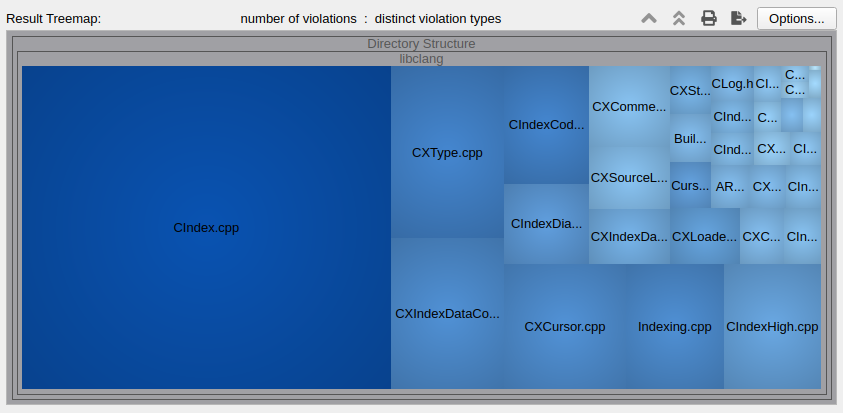
\includegraphics[width=\textwidth]{img/AllChecksTreeMap.png}
	\captionof{figure}{Result Treemap view.}
\end{minipage}
\vspace{1cm}

All the output perspectives can be exported in suitable formats (e.g. Treemap is exported in .png files while lists of violations are exported in .txt or .html files) that facilitate the second phase of the analysis.

\subsection{Understand Results}

As it has been said in the introduction, multiple analysis with different checks were ran:
\begin{itemize}
	\item[$a)$] MISRA-C++ 2008
	\item[$b)$] SciTools' Recommended Checks
	\item[$c)$] All Checks
	\item[$d)$] Clang Static Analyzer
\end{itemize}

\hspace{-0.6cm} \textbf{$a)$}  
This check is based on the MISRA-C++ 2008 standard, which is a standard developed for the quality of C++ source files.\newline
Results has been sorted by files and by MISRA rules. After that a compact view of these was produced showing the numbers of violations for each MISRA and for each file.\newline
Analyzing the reports it can be observed that:
\begin{itemize}
	\item The total number of violations in the \textbf{libclang} folder is 8450
	\item The first three rules that were violated the most are:
	\begin{itemize}
		\item[$1.\:$] MISRA08\_7-1-1 - \textbf{A variable which is not modified shall be const qualified} - 1845 violations.\newline If a variable does not need to be modified, then it shall be declared with const qualification so that it cannot be modified. A non-parametric variable will then require its initialization at the point of declaration. Also, future maintenance cannot accidentally modify the value.
		\item[$2.\:$] MISRA08\_6-4-1 - \textbf{An if condition construct shall be followed by a compund statement. The else keyword shall be followed by either a compound statement or another if statement} - 1239 violations.\newline If the bodies of these constructs are not compound statements, then errors can occur if a developer fails to add the required braces when attempting to change a single statement body to a multistatement body.
		Requiring that the body of these constructs shall be a compound statement (enclosed within braces) ensures that these errors cannot arise.
		\item[$3.\:$] MISRA08\_0-1-10 -\textbf{All defined functions called} - 733 violations.\newline Functions or procedures that are not called may be symptomatic of a serious problem, such as missing paths.
	\end{itemize}
	\item The first three files that contains the most violations are:
		\begin{itemize}
		\item[$1.\:$] CIndex.cpp - 3828 violations.
		\item[$2.\:$] CXType.cpp - 757 violations.
		\item[$3.\:$] CXCursor.cpp - 558 violations.
	\end{itemize}
\end{itemize}

Looking at the complete report, considerations can be made on the following aspects:

\begin{itemize}
	\item Some of the violations found (e.g. MISRA08\_0-1-10) include for sure some false-positive, due to the fact that the analysis was performed on a small subset of the complete project. Maybe the violation count for these rules could be reduced by performing a more comprehensive analysis.
	\item The violations distribution is reasonable, that is that most of the files have a similar issues count and the same can be said for MISRA rules.
	\item There is an exception both for files and for MISRA:
	\begin{itemize}
		\item[FILE: ] CIndex.cpp (3828 violations wrt 8450 total violations)
		\item[MISRA: ] MISRA08\_7-1-1 (1845 violations wrt 8450 total violations)
	\end{itemize}
	\item Using the Result Treemap feature it is possible to observe that the $NumberOfViolations/CountLineCode$ ratio varies between [0.27 - 1.75].
	\item Combining the use of the Result Treemap and Result Locator it is observable that the first 3 files in terms of $NumberOfViolations/CountLineCode$ ratio are relatively small files compared to the others.
	
\end{itemize}

\vspace{1cm}

\begin{minipage}{\linewidth}
	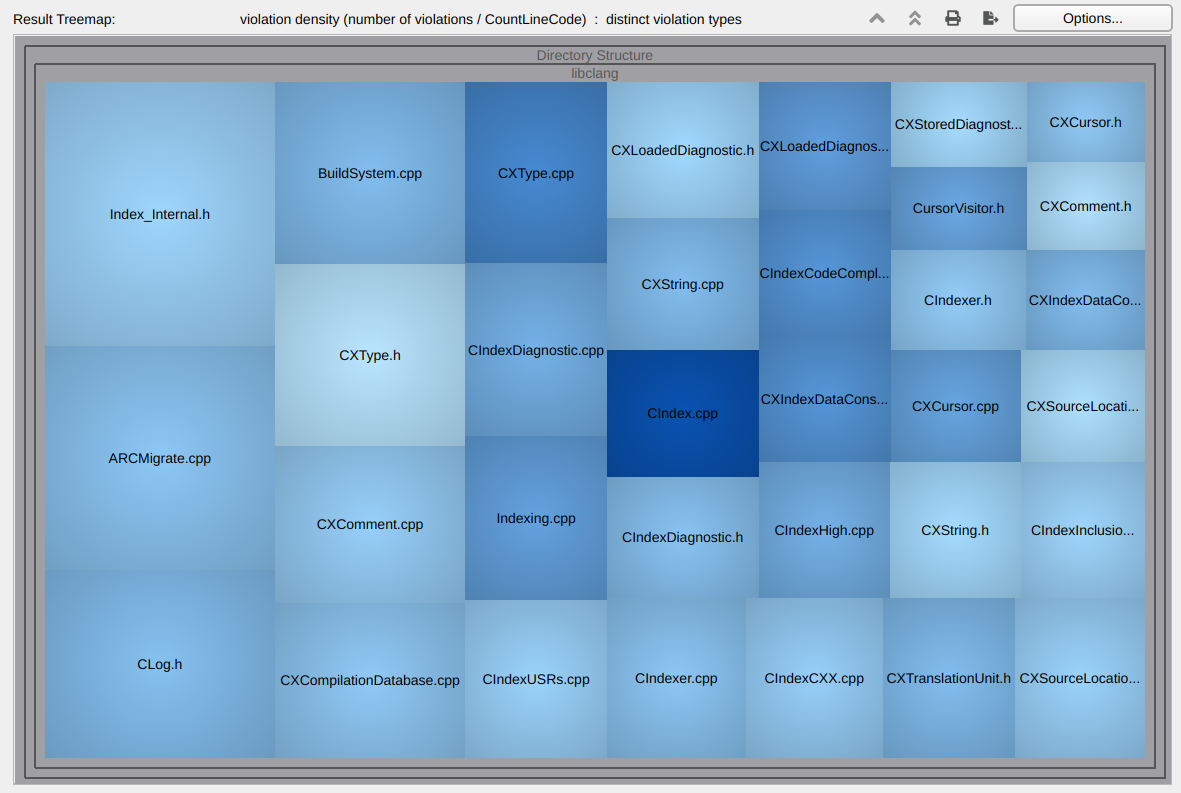
\includegraphics[width=\textwidth]{img/TreemapCountLine.png}
	\captionof{figure}{Result Treemap where files are sorted by $NumberOfViolations/CountLineCode$ ratio. Darker boxes indicates more distinct violation types while wider boxes indicate higher ratio.}
\end{minipage}
\pagebreak

\hspace{-0.6cm} \textbf{$b)$}  
SciTools Recommended Checks is a set of 17 quality checks based on code quality conventions that does not follow any precise standard.\newline
Results has been sorted by files and by the checkID provided by Understand. The postprocess phase was very similar to the previous one in order to obtain a compact view of data.\newline

\begin{itemize}
	\item The total number of violations in the \textbf{libclang} folder is 3299 (roughly 1000 violations less than the MISRA-check).
	\item The first three checks that were violated the most are:
	\begin{itemize}
		\item[$1.\:$] RECOMMENDED\_16 - \textbf{Each variable declaration should have a comment} - 1774 violations.\newline
		\item[$2.\:$] RECOMMENDED\_13 - \textbf{Every defined function shall be called at least once} - 733 violations.\newline 
		\item[$3.\:$] RECOMMENDED\_08 -\textbf{All fixed values will be defined constants} - 405 violations.\newline
	\end{itemize}
	\item The first three files that contains the most violations are:
		\begin{itemize}
		\item[$1.\:$] CIndex.cpp - 1472 violations.
		\item[$2.\:$] CXType.cpp - 266 violations.
		\item[$3.\:$] CXCursor.cpp - 250 violations.
	\end{itemize}
\end{itemize}

As it can be noticed by these data, the three files that have the most violations are the same as in the MISRA analysis.\newline
Looking at the complete dataset and comparing it to the previous one, the following considerations can be made:
\begin{itemize}
	\item The \textsl{RECOMMENDED\_13} plays a similar role as the MISRA08\_0-1-10. We can expect that when the analysis runs on the whole project the count number of this violation (\textsl{Every defined function shall be called at least once}) drops.
	\item The \textsl{RECOMMENDED\_16} check may seem too exaggerated but, if we think to big project as LLVM-Clang is, where multiple teams cooperate writing different chunks of code, this check become reasonable.
	\item The violations distribution with respect to files is quite odd. It can be observed that the average of the violations count is approximately 100. If we exclude the CIndex.cpp file the average drops approximately to 55.
	\item There is an exception both for files and for check, as we saw in the previous section:
	\begin{itemize}
		\item[FILE: ] CIndex.cpp (1472 violations wrt 3299 total violations)
		\item[MISRA: ] RECOMMENDED\_16(1774 violations wrt 3299 total violations)
	\end{itemize}
	\item Using the Result Treemap feature it is possible to observe that the $NumberOfViolations/CountLineCode$ ratio varies between [0.09 - 0.39].
\end{itemize}

\vspace{1cm}
\begin{minipage}{\linewidth}
	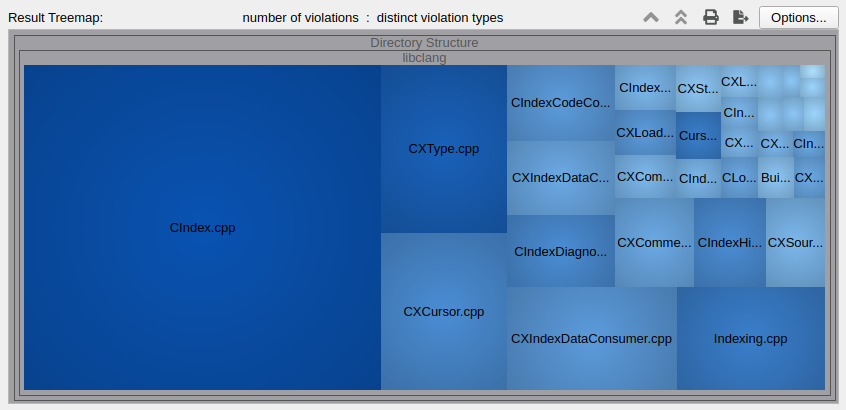
\includegraphics[width=\textwidth]{img/SciToolsViolationsCount.png}
	\captionof{figure}{Result Treemap where files are sorted by $NumberOfViolations$. As you can see the file CIndex.cpp covers almost half of the area.}
\end{minipage}
\pagebreak

\begin{minipage}{\linewidth}
	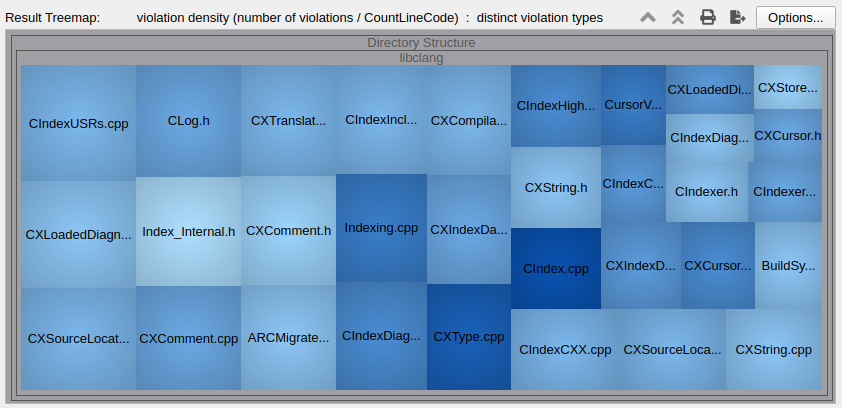
\includegraphics[width=\textwidth]{img/SciToolsViolationsRatio.png}
	\captionof{figure}{Despite the result in the previous figure, the $NumberOfViolations/LineOfCode$ ratio is quite homogeneous.}
\end{minipage}

\pagebreak

\hspace{-0.6cm} \textbf{$c)$}  
The \textsl{AllChecks} check set is the biggest among the provided ones. It includes most of the checks already seen in the previous sections, plus some completely new checks.\newline
Results has been sorted by files and by the checkID provided by Understand. The postprocess phase was very similar to the previous one in order to obtain a compact view of data.\newline

\begin{itemize}
	\item The total number of violations in the \textbf{libclang} folder is 30604 (indeed a very huge number compared to the previous ones).
	\item The first three checks that were violated the most are:
	\begin{itemize}
		\item[$1.\:$] CPP\_L000 - \textbf{Calls to COTS (Commercial Off The Shelf) library functions that might throw an exception, must be enclosed in a try block} - 5921 violations.\newline
		\item[$2.\:$] CPP\_I005 - \textbf{Identifier name reuse} - This check is concerned about variables' names. It requires that, in the same file, a different name is given to every different variable - 3546 violations.\newline 
		\item[$3.\:$] CPP\_V006 -\textbf{A variable which is not modified should be const qualified} - same as MISRA analysis - 1845 violations.\newline
	\end{itemize}
	\item The first three files that contains the most violations are:
		\begin{itemize}
		\item[$1.\:$] CIndex.cpp - 14004 violations.
		\item[$2.\:$] CXType.cpp - 2311 violations.
		\item[$3.\:$] CXIndexDataConsumer.cpp - 2078 violations.
	\end{itemize}
\end{itemize}

It is noticeable that, with this set of checks, the third file with most violations is \textsl{CXIndexDataConsumer.cpp} instead of \textsl{CIndex.cpp}.\newline
Let's now proceed with some considerations on this analysis as well:

\begin{itemize}
	\item Since this analysis include the previous ones, we assume that there are false-positives but they are caused mostly by the fact that the inspection was done on a subpart of the project. We don't have evidences of false-positives among the most common violations (see the complete excel report for more details).
	\item The most frequent violation is of a new kind. It is an important vulnerability that was pointed by none of the other analysis. This is quite odd since this is a quite important rule, well accepted by the developer community.
	\item The violations distribution with respect to files is similar to the previous ones.
	\item The violations distribution with respect to checks is almost uniformly distributed. This behaviour is gradually lost when the violations count goes over approximately 400)
	\item As well as the previous analysis, there is an exception both for files and for checks:
	\begin{itemize}
		\item[FILE: ] CIndex.cpp (14004 violations wrt 30604 total violations, almost half of the total)
		\item[MISRA: ] CPP\_L000(5921 violations wrt 30604 total violations. Recall that the second most common check had more than 2000 violations less)
	\end{itemize}
	\item Using the Result Treemap feature it is possible to observe that the $NumberOfViolations/CountLineCode$ ratio varies between [1 - 5.45]
\end{itemize}

\begin{minipage}{\linewidth}
	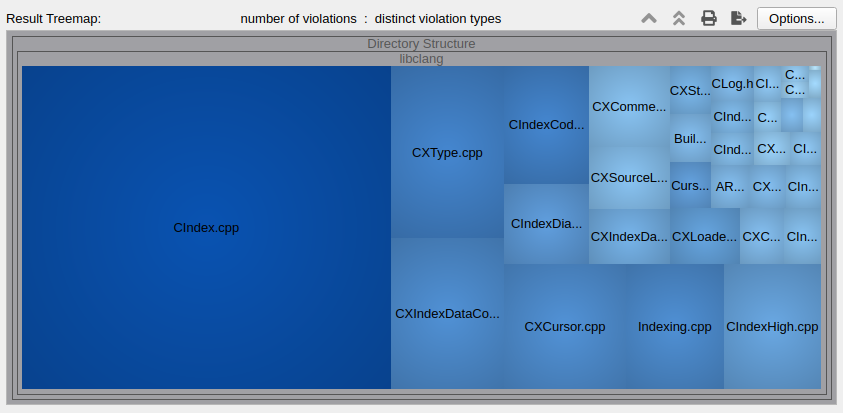
\includegraphics[width=\textwidth]{img/AllChecksTreeMap.png}
	\captionof{figure}{The CIndex.cpp file covers almost half of the total area also in this figure.}
\end{minipage}

\begin{minipage}{\linewidth}
	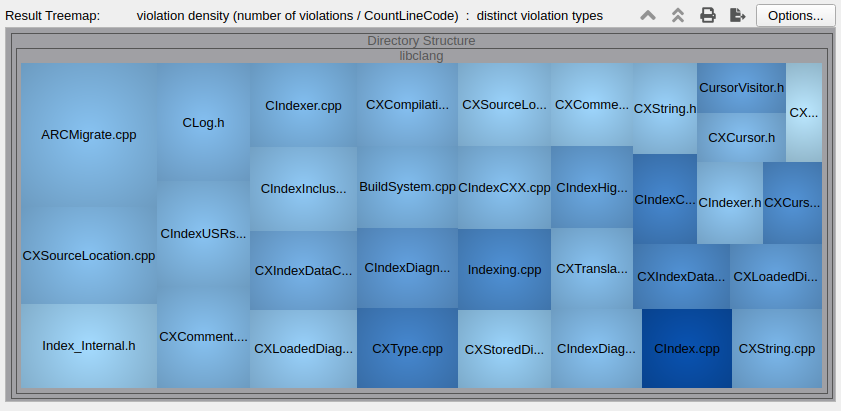
\includegraphics[width=\textwidth]{img/AllChecksViolationsRatio.png}
	\captionof{figure}{Even if the proportion of the $max/min$ of the ratio is similar to the previous, the ratio distribution itself is quite sparse (it ranges between 1 and 5.5), as well as the first analysis.}
\end{minipage}
\pagebreak

\hspace{-0.6cm} \textbf{$d)$}  
The \textsl{Clang Static Analyzer} check set is an implementation of the Clang Static Analyzer tool, developed as part of the LLVM-Clang project.\newline
The Clang Static Analyzer itself has not been used since it requires the build of the \textsl{whole} project to scan it. Moreover the increased knowledge of Understand and the presence of this set of checks embedded in the tool led us to the choice of using this implementation rather than the standalone tool.\newline\newline
This analysis did not find any violation. This seems reasonable since the metrics and quality practices chosen during the development of the LLVM-Clang compiler are probably the same metrics and checks implemented in the analyzer.

\subsection{Reports Summary}

In this conclusive section for the Understand analyzer, will be presented a summary of the most important observations along with some cross-checks. Summaries of the data collected throughout these analysis are reported at the end of the \textsl{Understand section}.\newline
\begin{itemize}

	\item All the analysis agreed that CIndex.cpp is the file with the largest violations count. The violations number of this file is usually very large, compared to the others.
	\item CXType.cpp is always the second file with the largest violations count. There are variations from the third position onwards, for example: CXCursor.cpp appears 2 times in the third position, while CXIndexDataConsumer.cpp appears 1 time.
	\item Looking at the $violationsCount/countLineCode$ ratio, it is observable that across the three analysis the $min/max$ proportion is very similar ($\approx 5.5 \pm 1$).
	\item It seems reasonable that using the metrics chosen by the project developers to analyze the source code no violations are found while, when different metrics are used, there are some violations.
	\item In some cases the violated metrics could be considered as a warning (e.g. to write a comment for every variable helps to keep the project well documented) while in some other cases (e.g. do not use try-catch construct) they are critical issues.
	\item Very likely, in these analyses, there are some false positives. This is because of the fact that the analyses were not performed on the whole project (e.g. functions that are never called in the analyzed modules could be called somewhere else).
	\item Some duplicated violations were reported when performing the analysis using the MISRA set. This is likely to be attributable to a possible overflow issue that has been noted also in the very first phase of the use of Understand. The duplicated issues had been removed in order to clean the dataset. No duplications were found using the other sets of rules.
\end{itemize}

\subsection{Understand Performances}

Understand is a very powerful tool, that comes with an easy-to-use user-interface and that gives a lot of informations about the performed analysis (e.g. result Treemap, result Locator, sort by check/file\dots)
On the other hand, it is not a lightweight program: we experienced unexpected crashes during analyses, issues duplication and a slow execution time in general. These are some of the main reasons that forced us to work on a subset of the LLVM-Clang compiler.\newline
Compared to the tools that will be presented in the next sections, this is indeed the most efficient in terms of \textsl{informations} and \textsl{versatility} (The various views it offers are a very powerful tool to navigate through the data). On the other hand, in terms of actual performance, it was the slowest one.

\pagebreak

\begin{minipage}{\linewidth}
	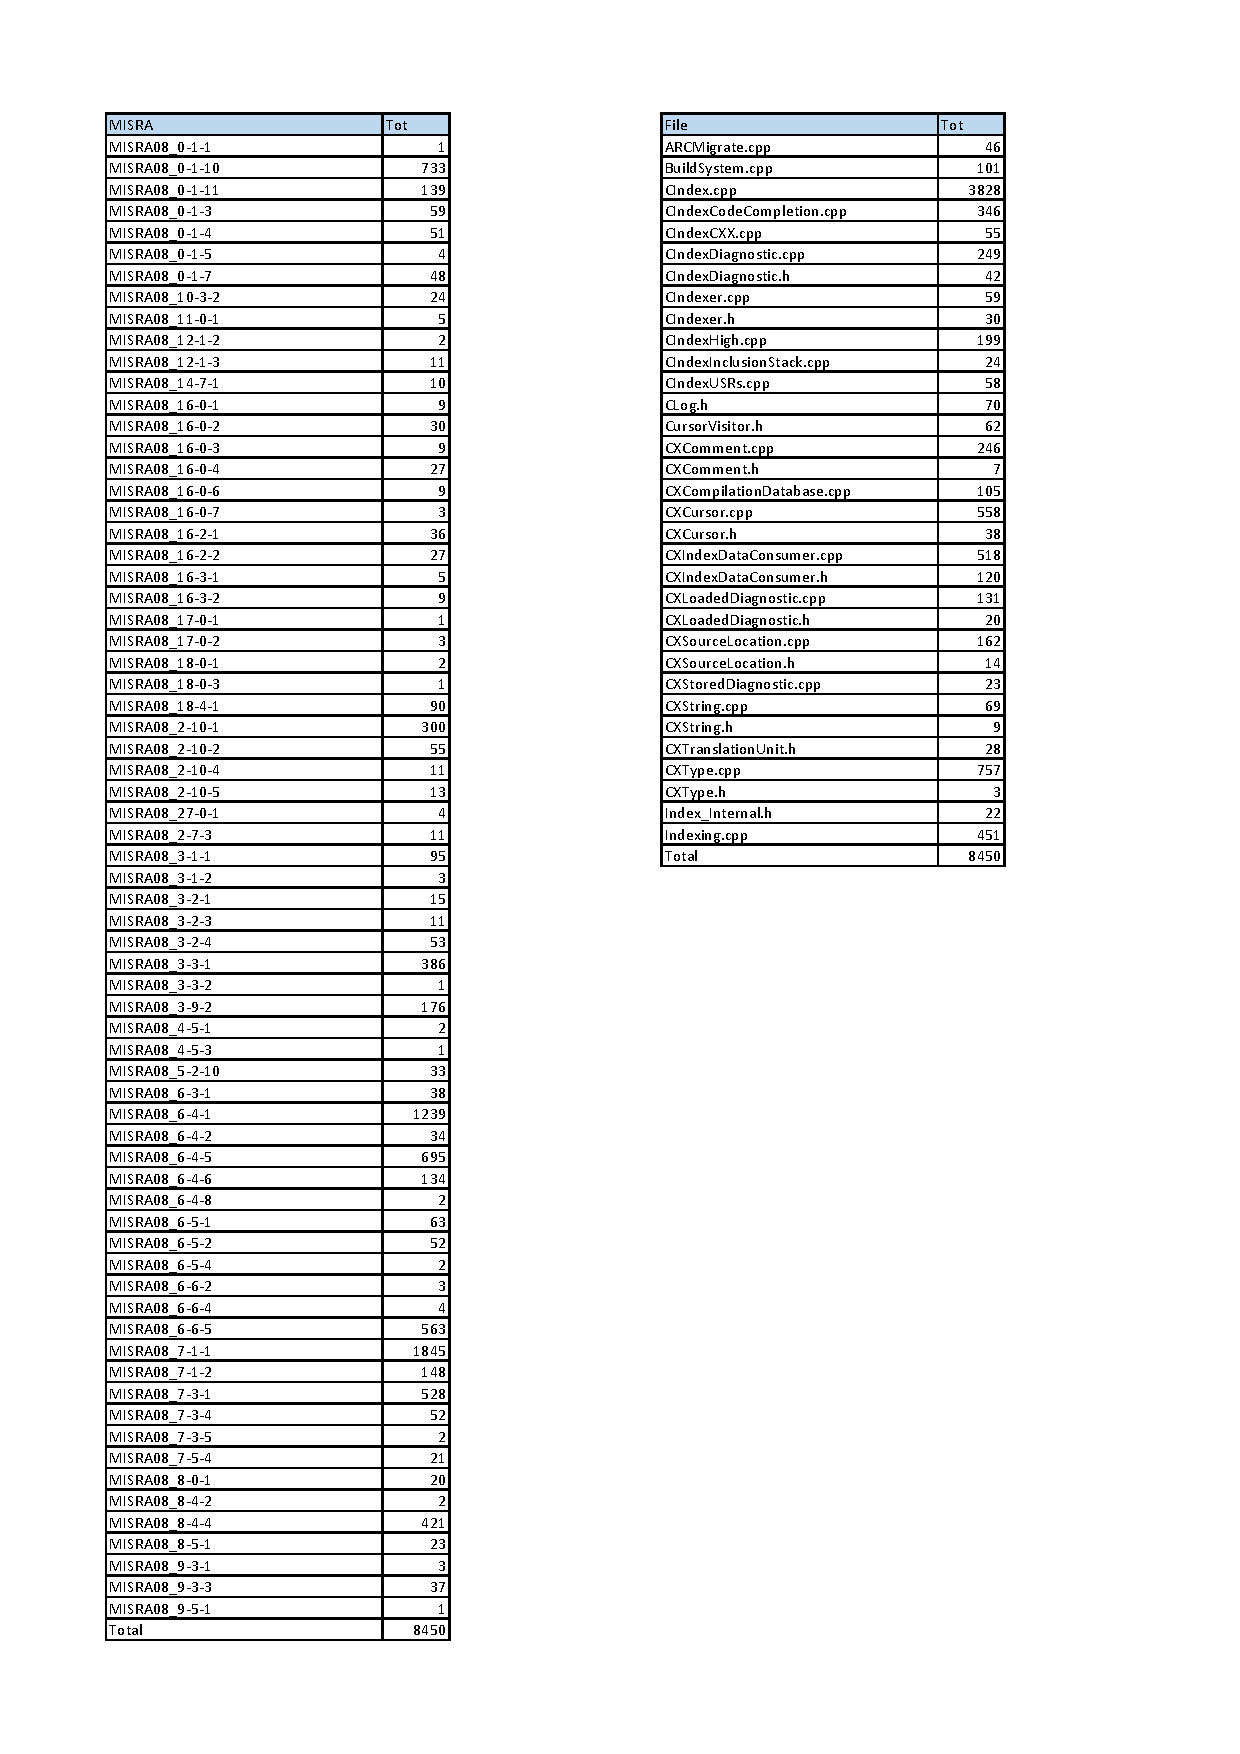
\includegraphics[width=\textwidth]{pdf/Misra_Summary.pdf}
	\captionof{figure}{Summary of the MISRA checks}
\end{minipage}

\pagebreak

\begin{minipage}{\linewidth}
	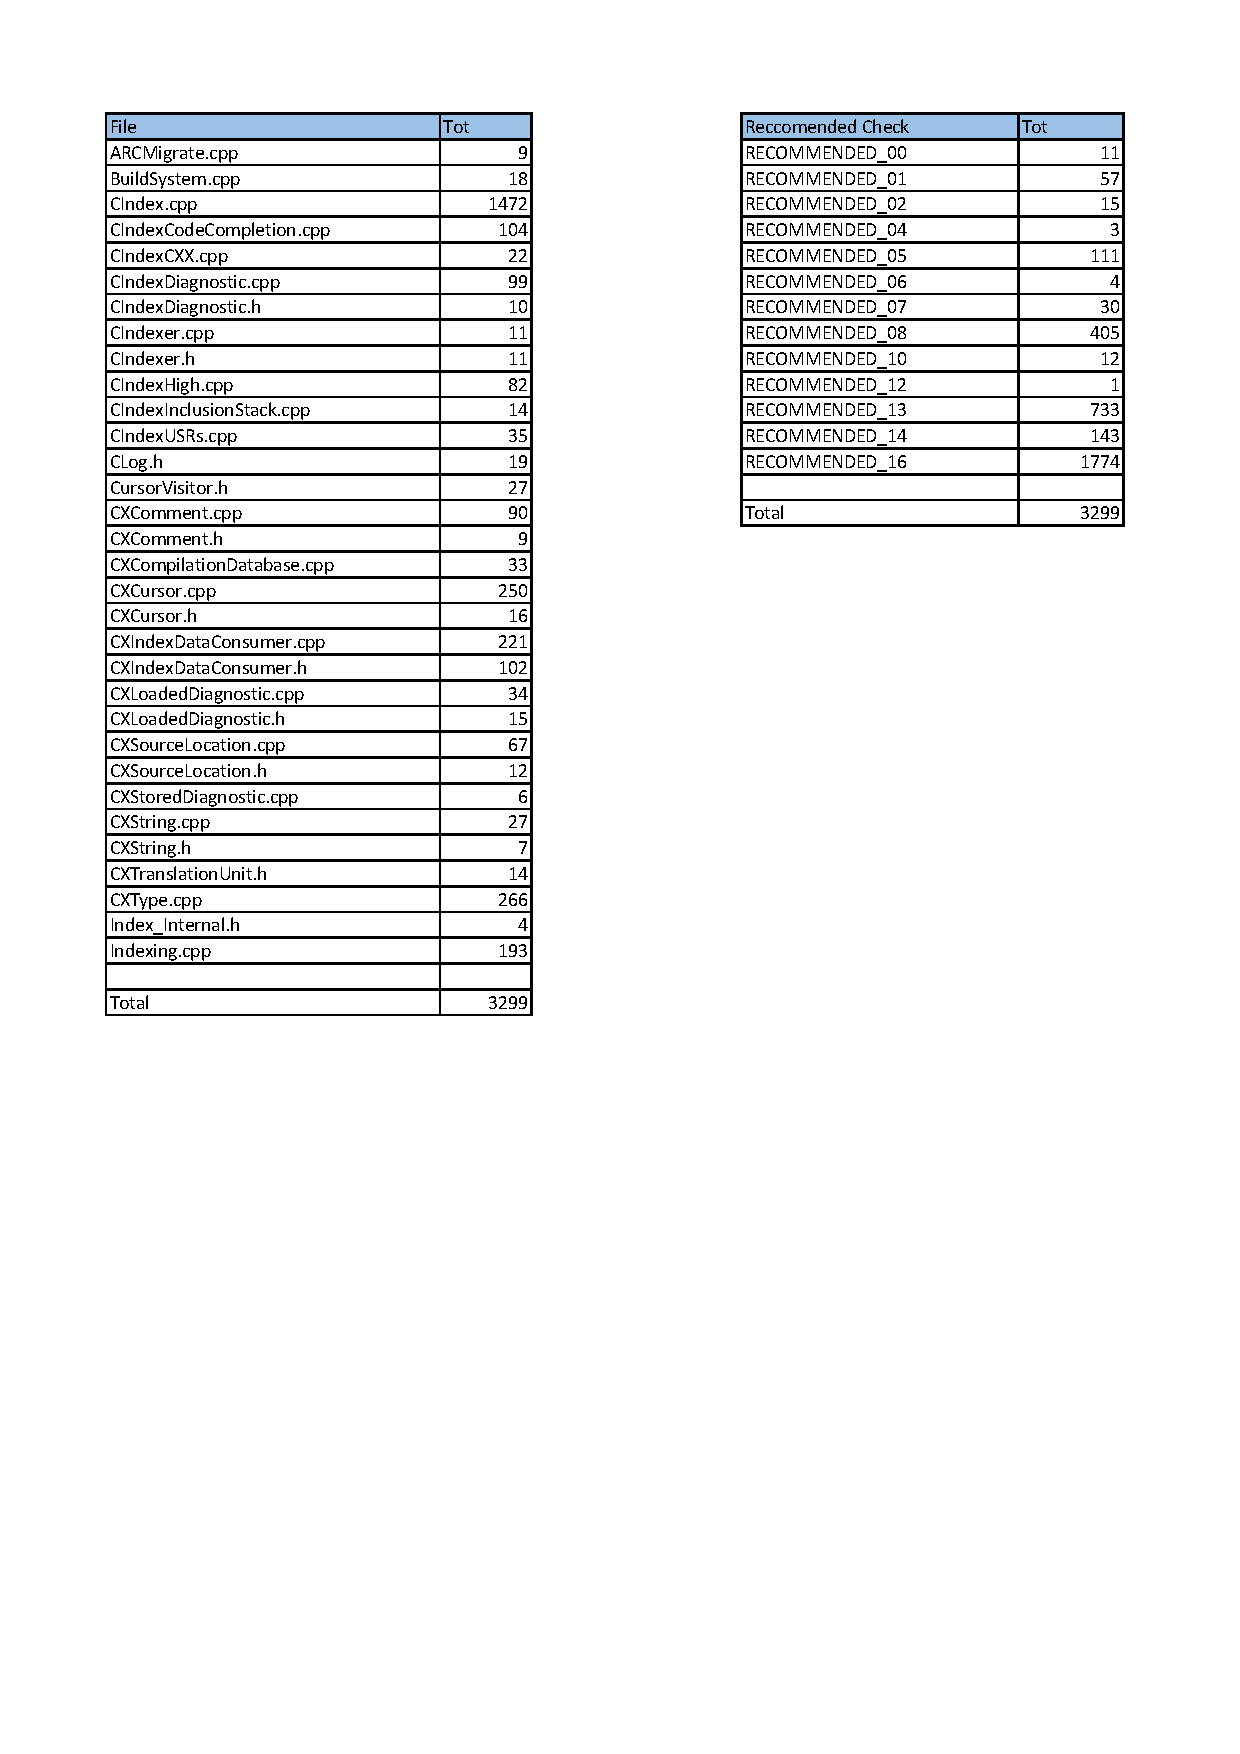
\includegraphics[width=\textwidth]{pdf/SciTools_Summary.pdf}
	\captionof{figure}{Summary of the SciTools Recommended Checks}
\end{minipage}

\pagebreak

\begin{minipage}{\linewidth}
	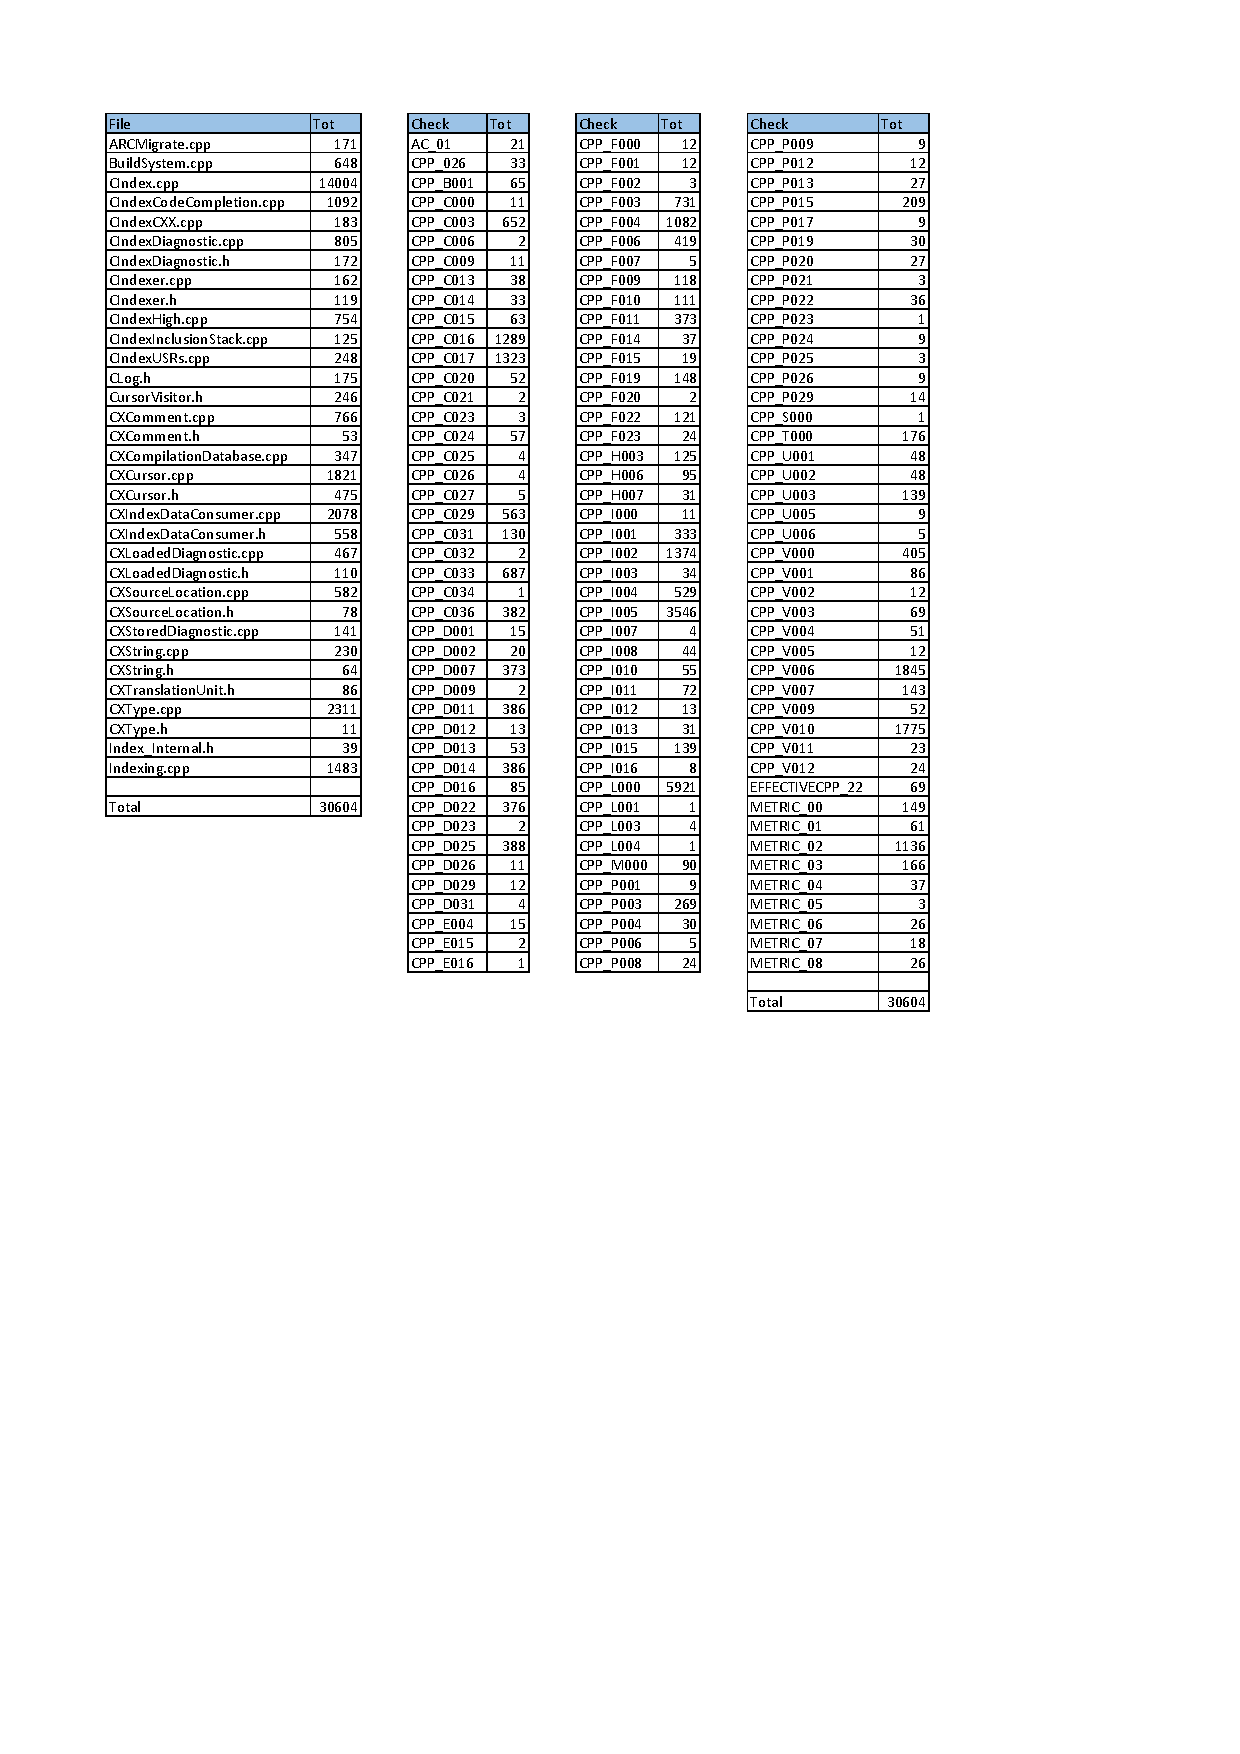
\includegraphics[width=\textwidth]{pdf/AllChecks_Summary.pdf}
	\captionof{figure}{Summary of the AllChecks checks}
\end{minipage}

\section{Cppcheck Analysis}

a